\documentclass[11pt,a4paper]{article}

\usepackage[margin=1in]{geometry}
\usepackage{booktabs}
\usepackage{longtable}
\usepackage{array}
\usepackage{graphicx}
\usepackage{xcolor}
\usepackage{listings}
\usepackage{amsmath}
\usepackage{amssymb}
\usepackage{enumitem}
\usepackage{natbib}
\usepackage{hyperref}

\hypersetup{
  colorlinks=true,
  linkcolor=blue!50!black,
  citecolor=blue!50!black,
  urlcolor=blue!50!black,
  bookmarksopen=true
}

\lstdefinestyle{pystyle}{
  language=Python,
  basicstyle=\ttfamily\small,
  keywordstyle=\color{blue!70!black}\bfseries,
  commentstyle=\color{gray!70!black}\itshape,
  stringstyle=\color{green!35!black},
  showstringspaces=false,
  breaklines=true,
  breakatwhitespace=false,
  columns=flexible,
  frame=single,
  rulecolor=\color{black!30},
  numbers=none,
  tabsize=4,
  xleftmargin=0.5em,
  xrightmargin=0.5em
}
\lstset{style=pystyle}

\newcommand{\pkg}{\texttt{pyxtabond2}}
\newcommand{\note}[1]{\par\medskip\noindent\fbox{\begin{minipage}{0.96\linewidth}\small\textbf{Note.} #1\end{minipage}}\medskip}
\newcommand{\warn}[1]{\par\medskip\noindent\fbox{\begin{minipage}{0.96\linewidth}\small\textbf{Caution.} #1\end{minipage}}\medskip}

\title{\textbf{PyXtabond2 User Manual}\\[0.4em]\Large Dynamic Panel GMM Estimation in Python}
\author{Frederic Kahindo}
\date{Version 0.0.2 --- \today}

\begin{document}

\maketitle

\begin{abstract}
\noindent \pkg{} is a Python package for estimating dynamic panel data
models by the Generalized Method of Moments (GMM), built to replicate the
matrix algebra, options, and diagnostics of Stata's \texttt{xtabond2}
\citep{Roodman2009a}. It covers Difference GMM \citep{ArellanoBond1991} and
System GMM \citep{ArellanoBover1995, BlundellBond1998}, one- and two-step
estimation with the \citet{Windmeijer2005} finite-sample correction, Forward
Orthogonal Deviations, instrument collapsing, and a full battery of
specification diagnostics. It also adds an original extension not present in
Stata's \texttt{xtabond2}: \emph{IFE-GMM}, an iterative PCA-based estimator
for dynamic panels contaminated by unobserved interactive fixed effects
\citep{Bai2009}, with an optional split-panel jackknife bias correction
\citep{DhaeneJochmans2015}. This manual documents the package's constructor options, diagnostics, export
paths, and known limitations as of v0.4.1. The underlying econometric theory, the line-by-line
validation against Stata, and the validity analysis of IFE-GMM are the
subject of a companion Methodological Note; this manual is deliberately
practical.
\end{abstract}

\tableofcontents

\section{Introduction}

\pkg{} targets applied econometricians who want a Python-native dynamic
panel GMM workflow without giving up the option surface and diagnostics that
Stata's \texttt{xtabond2} \citep{Roodman2009a} made a de facto standard. This
manual serves two audiences:

\begin{itemize}[nosep]
  \item Stata users porting a \texttt{xtabond2} specification to Python, who
        want a direct option-by-option mapping (Section~\ref{sec:mapping}).
  \item Researchers working with panels where unobserved \emph{common
        factors} (interactive fixed effects) are a concern, who want an
        estimator that purges them before GMM estimation (Section~\ref{sec:ife}).
\end{itemize}

\subsection{Key features}
\begin{itemize}[nosep]
  \item Difference GMM (Arellano-Bond) and System GMM (Blundell-Bond /
        Arellano-Bover), one-step and two-step, with all four
        robust/non-robust combinations Stata supports.
  \item \citet{Windmeijer2005} finite-sample correction for two-step robust
        standard errors.
  \item Forward Orthogonal Deviations \citep{ArellanoBover1995}, ideal for
        unbalanced panels with gaps.
  \item Full support for \textbf{unbalanced panels} -- missing
        \texttt{(id, time)} rows, not just missing values inside an
        existing row -- throughout estimation, in both the standard GMM
        engine and IFE-GMM (Section~\ref{sec:panels}).
  \item Instrument collapsing to control instrument proliferation
        \citep{Roodman2009b}.
  \item Generalized \texttt{h()}, \texttt{artests()}, \texttt{arlevels}, and
        single-variable \texttt{cluster()} options, matching \texttt{xtabond2.mata}.
  \item Per-variable-group instrument suboptions (\texttt{lag()},
        \texttt{collapse}, \texttt{eq()}) via \texttt{GMMStyle}/\texttt{IVStyle}.
  \item \textbf{IFE-GMM}: an original iterative PCA-defactoring GMM
        estimator for panels with interactive fixed effects
        \citep{Bai2009}, with automatic factor-count selection
        \citep{BaiNg2002, AhnHorenstein2013} and a split-panel jackknife
        bias correction \citep{DhaeneJochmans2015}.
  \item Publication-ready export to \LaTeX{} and Microsoft Word, including
        multi-model comparison tables.
\end{itemize}

\subsection{Package status}
\pkg{} is at version 0.4.1 (pre-1.0): the API may still change between minor
versions as features are added. Supported Python versions are 3.9--3.12.
Every numeric feature described in this manual has been cross-checked
against a fixed regression-fixture suite and, where a Stata equivalent
exists, against a real Stata run of \texttt{xtabond2} on the same data; see
the companion Methodological Note for the full validation record. (The
underlying \texttt{tests/} and \texttt{stata\_validation/} material lives in
the project's development repository and is not necessarily included in
every source distribution.)

\section{Installation}

\begin{lstlisting}[style=pystyle]
pip install pyxtabond2
\end{lstlisting}

Word export needs the optional \texttt{export} extra (the bundled example
datasets are plain CSV and need no extra dependency):
\begin{lstlisting}[style=pystyle]
pip install "pyxtabond2[export]"
\end{lstlisting}

Development install from source:
\begin{lstlisting}[style=pystyle]
git clone https://github.com/Kahindo048/pyxtabond2.git
cd pyxtabond2
pip install -e ".[dev,export]"
\end{lstlisting}

\begin{longtable}{@{}p{0.3\linewidth}p{0.25\linewidth}p{0.39\linewidth}@{}}
\toprule
\textbf{Dependency} & \textbf{Minimum version} & \textbf{Role} \\
\midrule
\endhead
numpy & 1.21 & Linear algebra core \\
pandas & 1.3 & Panel data handling \\
scipy & 1.7 & SVD, distributions \\
statsmodels & 0.13 & Summary table formatting \\
matplotlib & 3.5 & Factor-selection plots \\
numba & 0.56 & JIT-compiled panel transforms \\
\midrule
python-docx (extra: export) & 0.8 & Word export \\
pytest (extra: dev) & 7.0 & Test suite \\
\bottomrule
\end{longtable}

\section{Quick start}

\pkg{} bundles example datasets so you can experiment immediately.

\begin{lstlisting}[style=pystyle]
from pyxtabond2 import PanelData, PyXtabond2, load_dataset

# 1. Load the data
df = load_dataset('df_panel.csv')

# 2. Prepare the panel and precompute the lagged dependent variable
#    (Python has no live L./D. operators inside the estimation call --
#    lags used as *regressors* must be precomputed and merged in).
panel = PanelData(df, id_col='Country', time_col='Year')
panel.data['L1_Growth'] = panel.get_lag('Growth', 1)
df_ready = panel.data.reset_index()

# 3. Specify and estimate the model
model = PyXtabond2(
    df_ready,
    id_col='Country', time_col='Year', dep_var='Growth',
    x_vars=['L1_Growth', 'Capital', 'Labor', 'Wage', 'Investment', 'Ide'],
    gmm_vars=['Growth', 'Capital'],   # Arellano-Bond (GMM-style) instruments
    iv_vars=['Ide'],                  # standard IV instruments
    model_type='system', twostep=True, robust=True, small=True,
)
result = model.fit()
result.summary()

# 4. Export for publication
result.to_latex("gmm_results.tex", full_output=False)
result.to_word("gmm_results.docx", full_output=False)
\end{lstlisting}

See Section~\ref{sec:examples} for the full four-specification workflow
shipped as \texttt{examples.py} (in \texttt{examples/}).

\section{Preparing panel data: \texttt{PanelData}}
\label{sec:panels}

\texttt{PanelData} is the equivalent of Stata's \texttt{tsset}: it sorts the
data by (\texttt{id\_col}, \texttt{time\_col}), builds a \texttt{MultiIndex},
drops rows with a missing identifier or time period (with a warning), and
precomputes per-group row slices used throughout estimation.

\begin{lstlisting}[style=pystyle]
panel = PanelData(df, id_col='Country', time_col='Year')
panel.data                       # cleaned, sorted, MultiIndexed DataFrame
\end{lstlisting}

Three within-group temporal operators are provided, all NaN-aware (a group
with gaps does not contaminate a neighbouring group, and missing values
inside a group are simply skipped rather than propagated):

\begin{longtable}{@{}p{0.3\linewidth}p{0.67\linewidth}@{}}
\toprule
\textbf{Method} & \textbf{Description} \\
\midrule
\endhead
\texttt{get\_lag(var, lags=1)} & Stata's \texttt{L.var} / \texttt{L2.var}. \\
\texttt{get\_first\_difference(var)} & Stata's \texttt{D.var}. \\
\texttt{get\_fod(var)} & Arellano-Bover (1995) forward orthogonal
  deviations: subtracts the average of all \emph{available future}
  observations (rather than just the previous one), minimizing data loss in
  unbalanced panels with gaps. \\
\bottomrule
\end{longtable}

\warn{Python has no live \texttt{L.}/\texttt{D.} operator evaluated at
estimation time. Lags of the dependent variable that you want to use as a
\emph{regressor} (e.g.\ \texttt{L1\_Growth} in \texttt{x\_vars}) must be
precomputed with \texttt{get\_lag} and merged into the dataframe you pass to
\texttt{PyXtabond2}, as in the Quick Start above. This is distinct from the
GMM-style instruments generated automatically for \texttt{gmm\_vars}/\texttt{gmm}
(their own internal lag structure is built by \texttt{SystemGMMBuilder} and
needs no manual precomputation).}

\note{Panels with missing \texttt{(id, time)} rows (an individual skipping a
period entirely, joining late, or leaving early) are fully supported
throughout estimation -- by the temporal operators above, the GMM engine,
and IFE-GMM alike -- mirroring Stata \texttt{xtabond2}'s own internal
dense-grid handling of unbalanced data. No option is needed: gaps are
detected automatically from \texttt{id\_col}/\texttt{time\_col}.}

\section{The \texttt{PyXtabond2} estimator}
\label{sec:estimator}

\subsection{Overview}

\texttt{PyXtabond2} is the single entry point for every model the package
supports. Construct it with your data and specification, then call
\texttt{.fit()}:

\begin{lstlisting}[style=pystyle]
model = PyXtabond2(df, id_col, time_col, dep_var, x_vars, ...)
result = model.fit()   # -> PyXtabond2Results (Section 7)
\end{lstlisting}

\texttt{.fit()} routes automatically: if \texttt{r=0} (the default), it runs
the standard GMM engine directly; if \texttt{r} is a positive integer or
\texttt{'auto'}, it runs the IFE-GMM iterative loop instead
(Section~\ref{sec:ife}). Every other option below applies identically in
both cases.

\subsection{Core data parameters}

\texttt{df}, \texttt{id\_col}, \texttt{time\_col}, \texttt{dep\_var}, and
\texttt{x\_vars} specify, respectively: the panel (long format, one row per
unit-period), the cross-sectional identifier column, the time column, the
dependent variable, and the list of strictly exogenous regressors (which may
include precomputed lags, as above). These are the only five required,
positional arguments.

\subsection{Instrument specification}
\label{sec:instruments}

Two variable roles map onto Stata's two instrument families:

\begin{itemize}[nosep]
  \item \textbf{GMM-style instruments} (\texttt{gmm\_vars} / \texttt{gmm}):
        Arellano-Bond-style instruments built from a variable's own lags
        (endogenous or predetermined variables).
  \item \textbf{Standard IV instruments} (\texttt{iv\_vars} / \texttt{iv}):
        a variable used as its own instrument (strictly exogenous variables).
\end{itemize}

Each family has a flat \emph{shortcut} form and an advanced \emph{per-group}
form; the advanced form takes precedence when given.

\paragraph{Shortcut form.} \texttt{gmm\_vars} (list of column names) plus a
single \texttt{lag\_limits\_diff} (default \texttt{(2, None)}, meaning "lags
2 to the maximum available") and a single \texttt{collapse} flag (default
\texttt{False}) apply uniformly to every GMM-style variable. \texttt{iv\_vars}
is just a list of column names.

\paragraph{Advanced per-group form.} Pass \texttt{gmm=[GMMStyle(...), ...]}
and/or \texttt{iv=[IVStyle(...), ...]} to control lag windows, collapsing,
and equation targeting \emph{per variable group}, mirroring Stata's repeated
\texttt{gmm()}/\texttt{iv()} option syntax:

\begin{lstlisting}[style=pystyle]
from pyxtabond2 import GMMStyle, IVStyle

model = PyXtabond2(
    df, id_col='country_id', time_col='Year', dep_var='Growth',
    x_vars=['L.Growth', 'Capital', 'Labor', 'Wage', 'Investment', 'Ide'],
    gmm=[
        GMMStyle('Growth', lag=(2, 4), collapse=True),
        GMMStyle('Capital', lag=(2, None)),
    ],
    iv=[IVStyle('Ide')],
    model_type='system',
)
\end{lstlisting}

This reproduces (exactly, cross-checked against a real Stata run) Stata's
\texttt{gmm(Growth, lag(2 4) collapse) gmm(Capital, lag(2 .)) iv(Ide)}.

\begin{longtable}{@{}p{0.22\linewidth}p{0.15\linewidth}p{0.57\linewidth}@{}}
\toprule
\textbf{\texttt{GMMStyle} field} & \textbf{Default} & \textbf{Meaning} \\
\midrule
\endhead
\texttt{variables} & required & Variable(s) in this group (str or list). \\
\texttt{lag} & \texttt{(2, None)} & \texttt{(min\_lag, max\_lag)};
  \texttt{None} means "as many as available" (Stata's \texttt{.}). \\
\texttt{collapse} & \texttt{False} & Collapse into one instrument column per
  lag distance instead of one per (time period $\times$ lag). \\
\texttt{equation} & \texttt{"both"} & \texttt{"both"}, \texttt{"diff"}, or
  \texttt{"level"} -- which equation(s) this group instruments. Only
  meaningful for \texttt{model\_type='system'} (see caution below). \\
\bottomrule
\end{longtable}

\begin{longtable}{@{}p{0.22\linewidth}p{0.15\linewidth}p{0.57\linewidth}@{}}
\toprule
\textbf{\texttt{IVStyle} field} & \textbf{Default} & \textbf{Meaning} \\
\midrule
\endhead
\texttt{variables} & required & Variable(s) in this group. \\
\texttt{equation} & \texttt{"both"} & Same as \texttt{GMMStyle.equation}. \\
\bottomrule
\end{longtable}

\warn{Under \texttt{model\_type='difference'}, \texttt{GMMStyle.equation} is
always silently ignored: Difference GMM only ever has a differenced
equation, so there is nothing to select between. \texttt{IVStyle.equation}
follows the same rule for \texttt{"diff"} and \texttt{"both"}, but
\texttt{IVStyle(..., equation="level")} raises a \texttt{ValueError} instead
of being ignored, since it would leave the instrument assigned to no
equation at all. Use \texttt{"diff"} (or the default \texttt{"both"}) for any
\texttt{IVStyle} group under Difference GMM. \texttt{equation} only
meaningfully selects between equations for \texttt{model\_type='system'}.}

\note{Stata's further \texttt{passthru}, \texttt{mz}, and \texttt{split}
suboptions of \texttt{gmm()}/\texttt{iv()} are \textbf{not implemented} (see
Section~\ref{sec:limitations}).}

\subsection{Model type and estimation method}
\label{sec:modeltype}

\begin{longtable}{@{}p{0.18\linewidth}p{0.16\linewidth}p{0.58\linewidth}@{}}
\toprule
\textbf{Parameter} & \textbf{Default} & \textbf{Meaning} \\
\midrule
\endhead
\texttt{model\_type} & \texttt{'difference'} & \texttt{'difference'}:
  Arellano-Bond \citep{ArellanoBond1991}. \texttt{'system'}: Blundell-Bond /
  Arellano-Bover \citep{ArellanoBover1995, BlundellBond1998}, adding the
  levels equation instrumented by lagged differences. \\
\texttt{twostep} & \texttt{False} & Two-step efficient GMM instead of
  one-step. \\
\texttt{robust} & \texttt{False} & Robust (sandwich) standard errors;
  combined with \texttt{twostep}, applies the \citet{Windmeijer2005}
  finite-sample correction. \\
\texttt{orthogonal} & \texttt{False} & Forward Orthogonal Deviations instead
  of first differences. \\
\texttt{small} & \texttt{False} & Small-sample degrees-of-freedom
  corrections: $t$/$F$ statistics instead of $z$/$\chi^2$. \\
\bottomrule
\end{longtable}

\texttt{twostep} and \texttt{robust} combine into four distinct estimators,
exactly as in Stata:

\begin{longtable}{@{}p{0.12\linewidth}p{0.12\linewidth}p{0.35\linewidth}p{0.31\linewidth}@{}}
\toprule
\textbf{twostep} & \textbf{robust} & \textbf{Estimator} & \textbf{Variance source} \\
\midrule
\endhead
False & False & One-step, non-robust (homoscedastic) & Analytic $V_1$ scaled
  by an estimated error variance $\hat\sigma^2$. \\
False & True & One-step, robust (sandwich) & Robust sandwich $V_{1,\mathrm{rob}}$;
  the Hansen test is additionally obtained via a silent two-step-style refit
  ("Roodman's trick"), without altering the reported one-step $\hat\beta$/se. \\
True & False & Two-step, non-robust (rare) & $\sqrt{\mathrm{diag}(V_2)}$, no
  Windmeijer correction -- Stata allows this combination but it is seldom
  used in practice. \\
True & True & Two-step, robust = \citet{Windmeijer2005} & Windmeijer-corrected
  $V_{2,\mathrm{robust}}$ -- the estimator most commonly reported in applied
  work. \\
\bottomrule
\end{longtable}

\note{\textbf{System GMM automatically adds a constant.} When
\texttt{model\_type='system'}, a constant term (\texttt{\_cons}) is
automatically appended to the regressors and instrumented in the levels
equation -- you do not need to (and should not) add it to \texttt{x\_vars}
yourself. Difference GMM never has a constant term, since it cancels
identically under differencing (matching Stata exactly). You will see
\texttt{\_cons} appear in the coefficient table of any System GMM result.}

\subsection{Weighting-matrix and test controls}
\label{sec:weighting}

\begin{longtable}{@{}p{0.16\linewidth}p{0.12\linewidth}p{0.66\linewidth}@{}}
\toprule
\textbf{Parameter} & \textbf{Default} & \textbf{Meaning} \\
\midrule
\endhead
\texttt{h} & \texttt{3} & One-step weighting-matrix structure (Stata's
  \texttt{h()}). \texttt{h=3} (default) models the known cross-covariance
  between the differenced/orthogonal-deviations equation and the levels
  equation. \texttt{h=2} assumes that cross-covariance is zero. \texttt{h=1}
  assumes no serial-correlation structure at all (identity weighting).
  \texttt{h=1}/\texttt{h=2} are rarely needed in practice; \texttt{h=2} and
  \texttt{h=3} coincide for pure Difference GMM. \\
\texttt{artests} & \texttt{2} & Highest-order Arellano-Bond AR($\ell$)
  serial-correlation test reported (default: AR(1) and AR(2)). Raise this to
  probe higher-order serial correlation directly. \\
\texttt{arlevels} & \texttt{False} & If \texttt{True}, the AR($\ell$) tests
  target the \emph{levels}-equation residuals instead of the
  differenced/orthogonal-deviations residuals. Only valid for
  \texttt{model\_type='system'} (raises \texttt{ValueError} otherwise). \\
\texttt{cluster} & \texttt{None} & Column name to cluster the robust/two-step
  variance matrix by, instead of the default panel id. \textbf{Single
  variable only} -- see Section~\ref{sec:limitations} for the multi-way
  limitation and a numerical caveat when instruments outnumber clusters. \\
\bottomrule
\end{longtable}

\subsection{IFE-GMM parameters (overview)}

\texttt{r}, \texttt{r\_max}, \texttt{ife\_max\_iter}, \texttt{ife\_tol}, and
\texttt{bias\_correction} control the original IFE-GMM extension and are
detailed in full in Section~\ref{sec:ife}; \texttt{r=0} (the default) simply
disables IFE-GMM and every model in this manual up to that point uses
standard GMM.

\subsection{Full parameter reference}
\label{sec:fullref}

\begin{longtable}{@{}p{0.21\linewidth}p{0.15\linewidth}p{0.13\linewidth}p{0.41\linewidth}@{}}
\toprule
\textbf{Parameter} & \textbf{Type} & \textbf{Default} & \textbf{Description} \\
\midrule
\endhead
\texttt{df} & DataFrame & required & Panel dataset (long format). \\
\texttt{id\_col} & str & required & Cross-sectional identifier column. \\
\texttt{time\_col} & str & required & Time-period column. \\
\texttt{dep\_var} & str & required & Dependent variable. \\
\texttt{x\_vars} & list[str] & required & Strictly exogenous regressors. \\
\texttt{gmm\_vars} & list[str] & \texttt{None} & Shortcut GMM-style
  instrument variables (single group). \\
\texttt{iv\_vars} & list[str] & \texttt{None} & Shortcut standard-instrument
  variables (single group). \\
\texttt{model\_type} & str & \texttt{'difference'} & \texttt{'difference'}
  or \texttt{'system'}. \\
\texttt{twostep} & bool & \texttt{False} & Two-step instead of one-step GMM. \\
\texttt{robust} & bool & \texttt{False} & Robust/Windmeijer standard errors. \\
\texttt{lag\_limits\_diff} & tuple & \texttt{(2, None)} & Shortcut lag window
  for \texttt{gmm\_vars}. \\
\texttt{collapse} & bool & \texttt{False} & Shortcut collapse flag for
  \texttt{gmm\_vars}. \\
\texttt{gmm} & list[GMMStyle] & \texttt{None} & Advanced per-group GMM-style
  instruments; overrides the shortcuts above. \\
\texttt{iv} & list[IVStyle] & \texttt{None} & Advanced per-group standard
  instruments; overrides \texttt{iv\_vars}. \\
\texttt{orthogonal} & bool & \texttt{False} & Forward Orthogonal Deviations
  instead of first differences. \\
\texttt{small} & bool & \texttt{False} & Small-sample dof corrections
  ($t$/$F$ vs.\ $z$/$\chi^2$). \\
\texttt{r} & int or 'auto' & \texttt{0} & Number of IFE-GMM factors; 0 =
  plain GMM. \\
\texttt{r\_max} & int & \texttt{5} & Max factors tested when
  \texttt{r='auto'}. \\
\texttt{ife\_max\_iter} & int & \texttt{30} & Max IFE-GMM loop iterations. \\
\texttt{ife\_tol} & float & \texttt{1e-5} & IFE-GMM convergence tolerance. \\
\texttt{bias\_correction} & bool & \texttt{False} & Split-panel jackknife
  bias correction on top of IFE-GMM. \\
\texttt{h} & \{1,2,3\} & \texttt{3} & One-step weighting-matrix structure. \\
\texttt{artests} & int & \texttt{2} & Highest AR($\ell$) lag tested. \\
\texttt{arlevels} & bool & \texttt{False} & AR($\ell$) tests on levels
  residuals (system only). \\
\texttt{cluster} & str & \texttt{None} & Single clustering variable for
  robust/two-step inference. \\
\bottomrule
\end{longtable}

\section{Python \texorpdfstring{$\leftrightarrow$}{<->} Stata \texttt{xtabond2} option mapping}
\label{sec:mapping}

\warn{\textbf{Default model type differs.} \pkg{}'s own default is
\texttt{model\_type='difference'}. Stata's \texttt{xtabond2} default is
\emph{System} GMM (the level equation is included unless \texttt{noleveleq}
is given). A direct Stata-to-Python port therefore needs
\texttt{model\_type='system'} explicitly unless the Stata call used
\texttt{noleveleq}.}

\begin{longtable}{@{}p{0.32\linewidth}p{0.32\linewidth}p{0.30\linewidth}@{}}
\toprule
\textbf{\pkg{}} & \textbf{Stata \texttt{xtabond2}} & \textbf{Notes} \\
\midrule
\endhead
\texttt{model\_type='system'} & default (no \texttt{noleveleq}) & See
  caution above: opposite defaults. \\
\texttt{model\_type='difference'} & \texttt{noleveleq} & \pkg{}'s own default. \\
\texttt{gmm\_vars} / \texttt{gmm=[GMMStyle(...)]} & \texttt{gmm(varlist,
  lag(a b) collapse eq(diff|level|both))} & One \texttt{GMMStyle} group = one
  \texttt{gmm()} call; \texttt{lag=(a,b)} $\leftrightarrow$ \texttt{lag(a b)}
  (\texttt{None} $\leftrightarrow$ Stata's \texttt{.}). \\
\texttt{iv\_vars} / \texttt{iv=[IVStyle(...)]} & \texttt{iv(varlist, eq(diff|level|both))} &
  Analogous to \texttt{gmm()}. \\
\texttt{twostep} & \texttt{twostep} & Direct. \\
\texttt{robust} & \texttt{robust} & Direct, including the one-step
  "Roodman's trick" Hansen refit. \\
\texttt{orthogonal} & \texttt{orthogonal} & Direct (FOD vs.\ first
  differences). \\
\texttt{small} & \texttt{small} & Direct. \\
\texttt{h=1/2/3} & \texttt{h(1)}/\texttt{h(2)}/\texttt{h(3)} & Direct, same
  default (3). \\
\texttt{artests=\#} & \texttt{artests(\#)} & Direct, same default (2). \\
\texttt{arlevels} & \texttt{arlevels} & Direct, System-only in both. \\
\texttt{cluster=var} & \texttt{cluster(varname)} & \pkg{}: single variable
  only, \emph{not} Stata's multi-way \texttt{cluster(var1 var2)}. \\
\texttt{r}, \texttt{r\_max}, \texttt{ife\_max\_iter}, \texttt{ife\_tol},
  \texttt{bias\_correction} & \emph{no equivalent} & Original \pkg{}
  extension (IFE-GMM, Section~\ref{sec:ife}); not part of \texttt{xtabond2}.
  The closest Stata-world tools are the community-contributed
  \texttt{xtivdfreg} (two-stage defactored IV,
  \citealp{KripfganzSarafidis2021, Norkute2021}) or \texttt{xtdcce2} (Common
  Correlated Effects, \citealp{Ditzen2018, Pesaran2006}) -- different
  estimators, not drop-in equivalents. \\
\emph{not available} & \texttt{pweight}/\texttt{aweight}/\texttt{fweight} &
  Not implemented (Section~\ref{sec:limitations}). \\
\emph{not available} & multi-way \texttt{cluster(var1 var2)} & Not
  implemented (Section~\ref{sec:limitations}). \\
\emph{not available} & \texttt{gmm()}/\texttt{iv()}'s \texttt{passthru},
  \texttt{mz}, \texttt{split} suboptions & Not implemented. \\
\bottomrule
\end{longtable}

\section{Estimation results: \texttt{PyXtabond2Results}}
\label{sec:results}

\texttt{.fit()} returns a \texttt{PyXtabond2Results} instance.

\begin{longtable}{@{}p{0.22\linewidth}p{0.75\linewidth}@{}}
\toprule
\textbf{Attribute} & \textbf{Description} \\
\midrule
\endhead
\texttt{.beta}, \texttt{.se} & Coefficient and standard-error column vectors,
  aligned with \texttt{.x\_names}. \\
\texttt{.t\_stats}, \texttt{.p\_values} & $t$/$z$ statistics and two-sided
  $p$-values. \\
\texttt{.ci\_lower}, \texttt{.ci\_upper} & 95\% confidence interval bounds. \\
\texttt{.x\_names} & Regressor names, in output order (includes
  \texttt{\_cons} for System GMM). \\
\texttt{.diag} & Dictionary of diagnostic tests (see below); advanced use. \\
\texttt{.engine} & The underlying \texttt{GMMEngine}; advanced/internal use
  (raw matrices, group structure). \\
\bottomrule
\end{longtable}

\subsection{\texttt{.summary()}}

\texttt{result.summary()} prints a Stata-style report with four blocks:

\begin{enumerate}[nosep]
  \item \textbf{Header}: dependent variable, model/method, date/time,
        observation and group counts, obs.\ per group, instrument count,
        covariance type, the Wald/$F$ statistic and its $p$-value, and the
        active specification (GMM/IV variable lists, lag limits, collapse,
        FOD, small-sample correction).
  \item \textbf{Coefficient table}: coefficient, standard error, $t$/$z$
        statistic, $p$-value, and 95\% CI for each regressor.
  \item \textbf{Diagnostic Tests}: AR($\ell$) for $\ell=1,\dots,$
        \texttt{artests}, the Sargan test, and (when available) the Hansen
        test.
  \item \textbf{Difference-in-\{Sargan,Hansen\} Tests}: one row pair for the
        System GMM "GMM instruments for levels" block (when applicable),
        plus one further row pair covering all \texttt{iv()}/\texttt{iv\_vars}
        instruments jointly. Every standard-instrument variable, across every
        \texttt{IVStyle} group, is tested together as a single combined
        subset -- not group by group.
\end{enumerate}

\subsection{Interpreting the diagnostics}
\label{sec:diagdiag}

\begin{description}[nosep]
  \item[AR(1)/AR(2)] Arellano-Bond serial-correlation tests on the
    transformed-equation residuals ($H_0$: no serial correlation at that
    order). Differencing (or FOD) mechanically induces first-order
    correlation in well-specified errors, so \textbf{rejecting AR(1) is
    expected and not a problem}. Failing to reject AR(2) or higher, however,
    is required for validity of lag-2-and-beyond instruments; a rejected
    AR(2) signals that the original error term was itself serially
    correlated, invalidating those instruments. Raise \texttt{artests} to
    inspect AR(3), AR(4), \dots directly.
  \item[Sargan vs.\ Hansen] Both are overidentification tests of instrument
    validity ($H_0$: instruments are valid). The Sargan test is always
    computed but is only valid under homoskedasticity; the Hansen test is
    consistent under the active robust/two-step weighting matrix (available
    whenever \texttt{twostep} or \texttt{robust} is set, including the
    one-step-robust "Roodman's trick" case) and should be preferred when
    present. Both tests \textbf{lose power as instruments proliferate}
    \citep{Roodman2009b} -- a suspiciously high Hansen $p$-value (e.g.\
    $>0.99$) with many instruments is itself a warning sign rather than
    reassurance; consider \texttt{collapse=True}.
  \item[Difference-in-Sargan/Hansen] Tests the exogeneity of a specific
    instrument \emph{subset} by comparing the overidentification statistic
    with and without it. A large difference $p$-value supports treating that
    subset as valid on its own.
  \item[Wald / $F$ test] Joint significance of all regressors
    (\texttt{\_cons} excluded from the tested set and from its degrees of
    freedom when present). Reported as an $F$ statistic under
    \texttt{small=True}, as $\chi^2$ otherwise.
\end{description}

\section{Exporting results}
\label{sec:export}

\begin{lstlisting}[style=pystyle]
result.to_latex("table.tex", full_output=False)   # booktabs academic table
result.to_latex("appendix.tex", full_output=True)  # verbatim console capture
result.to_word("table.docx", full_output=False)    # requires pyxtabond2[export]
\end{lstlisting}

\texttt{full\_output=False} (default) produces a clean coefficients table
plus a diagnostics table, formatted with \texttt{booktabs} rules or native
Word table styles, suitable for direct inclusion in a paper. \texttt{full\_output=True}
instead captures the exact \texttt{.summary()} console output verbatim
(monospace), convenient for an appendix or a robustness-check log.

\subsection{Comparing multiple models: \texttt{GMMStargazer}}

\begin{lstlisting}[style=pystyle]
from pyxtabond2 import GMMStargazer

stargazer = GMMStargazer(
    [res1, res2, res3],
    model_names=["Diff (1-Step)", "Sys (1-Step)", "Sys (2-Step Robust)"],
)
stargazer.to_latex("comparison.tex")
stargazer.to_word("comparison.docx")
\end{lstlisting}

\texttt{GMMStargazer} builds a side-by-side comparison table (à la Stata's
\texttt{esttab}/\texttt{estout} or R's \texttt{stargazer}): it takes the
union of regressors, AR lags, and Diff-in-Sargan/Hansen tests across all
supplied models (models missing a given row show \texttt{-}), and marks
significance with $^{*}p{<}0.1$, $^{**}p{<}0.05$, $^{***}p{<}0.01$. See
Table~\ref{tab:fourmodel} (Section~\ref{sec:examples}) for a complete,
real four-model instance of exactly this table.

\section{IFE-GMM: the interactive-fixed-effects extension}
\label{sec:ife}

\subsection{Motivation}

Standard Arellano-Bond/Blundell-Bond GMM assumes the idiosyncratic error is
uncorrelated with the instruments. If the panel instead contains
\emph{unobserved common factors} with heterogeneous, unit-specific loadings
-- interactive fixed effects, in the sense of \citet{Bai2009} -- driving
both the regressors and the dependent variable, that assumption fails and
standard GMM is biased. IFE-GMM adds an iterative PCA-based defactoring step
around the same GMM engine: extract candidate factors from current
residuals, project the dependent variable, regressors, \emph{and}
instruments onto the space orthogonal to those factors, re-estimate GMM, and
repeat until the coefficient vector stabilizes.

\subsection{Parameters}

\begin{description}[nosep]
  \item[\texttt{r=0}] (default) Plain GMM; no defactoring. Identical to
    omitting IFE-GMM entirely.
  \item[\texttt{r=}\emph{int}] Fixed number of factors. Each iteration:
    residuals $\to$ SVD $\to$ extract the top $r$ factors $F$ ($T\times r$,
    normalized so $F'F/T = I_r$, following \citealp{Bai2009}) $\to$ project
    with $M_F = I_T - FF'/T$ $\to$ re-run GMM on the projected data $\to$
    check convergence.
  \item[\texttt{r='auto'}] Estimates the number of factors first, from the
    plain-GMM residuals reshaped into an $N\times T$ matrix, via the
    \citet{AhnHorenstein2013} eigenvalue-ratio criterion (with the
    \citet{BaiNg2002} $IC_{p2}$ criterion also computed and reported),
    mirroring Stata's \texttt{xtnumfac}, built using the same missing-cell
    handling described below.
  \item[\texttt{r\_max=5}] Caps the factor search when \texttt{r='auto'}.
  \item[\texttt{ife\_max\_iter=30}, \texttt{ife\_tol=1e-5}] Convergence-loop
    cap and tolerance on $\sum|\hat\beta_{\text{new}}-\hat\beta_{\text{old}}|$.
  \item[\texttt{bias\_correction=False}] Applies the
    \citet{DhaeneJochmans2015} split-panel jackknife on top of the converged
    IFE-GMM fit: split the panel in half along the \emph{time} dimension,
    re-run IFE-GMM on each half (warm-started from the full-panel solution),
    and combine as
    \[
      \hat\beta_{\mathrm{BC}} = 2\hat\beta_{\text{full}}
        - \tfrac{1}{2}\left(\hat\beta_{t\le\bar t} + \hat\beta_{t>\bar t}\right),
    \]
    correcting an $O(1/T)$ incidental-parameter-style asymptotic bias.
    Roughly doubles computation time (two half-panel refits).
\end{description}

\note{Any panel cell without a defined residual -- a genuine gap in an
unbalanced panel, or simply a variable's own first observation per unit
(an undefined lag) -- is filled automatically before each iteration's
factor extraction, using the \emph{previous} iteration's own rank-$r$
reconstruction (a cross-sectional mean on the very first iteration, before
one exists). \pkg{} prints an informational, one-time console notice the
first time this triggers per fit; it requires no user action and does not
change the structure of the returned result. See the companion
Methodological Note for the exact mechanism.}

\begin{lstlisting}[style=pystyle]
# Fixed factor count, with bias correction
model = PyXtabond2(df, id_col, time_col, dep_var, x_vars,
                    gmm_vars=['y'], iv_vars=['x1', 'x2'],
                    model_type='system', r=2, bias_correction=True)
result = model.fit()

# Automatic factor-count selection
model_auto = PyXtabond2(df, id_col, time_col, dep_var, x_vars,
                         gmm_vars=['y'], iv_vars=['x1', 'x2'],
                         model_type='system', r='auto', r_max=5)
result_auto = model_auto.fit()
model_auto.plot_factor_selection(mode='table')   # or mode='graph'
\end{lstlisting}

\texttt{plot\_factor\_selection} only works after fitting with
\texttt{r='auto'} (it reads criteria stored during that fit); it prints a
table (returns a \texttt{DataFrame}) or a two-panel plot of the ER/$IC_{p2}$
criteria across candidate factor counts (returns a \texttt{Figure}).

\note{During IFE-GMM fitting, progress is printed to the console (factor
count selected, per-iteration convergence delta, jackknife status). This is
informational only and does not affect the returned result.}

\subsection{Convergence and bias caveats}
\label{sec:ifecaveats}

Two structural limitations apply to IFE-GMM and are documented here rather
than silently assumed away (full theoretical treatment in the companion
Methodological Note):

\begin{enumerate}[nosep]
  \item \textbf{Convergence is not guaranteed from an inconsistent starting
    point.} \citet{HongSuJiang2022} prove fast contraction to the true
    parameter for exactly this update formula, but only from a starting
    estimate that is already consistent under factors (they obtain one via
    nuclear-norm regularization). \pkg{}'s loop instead starts from the
    plain (non-defactored) GMM fit, which is \emph{not} guaranteed consistent
    in the presence of strong factors. Empirically the loop tends to behave
    well, but convergence should be read as a good empirical sign, not a
    correctness proof, especially with dominant factors.
  \item \textbf{Without \texttt{bias\_correction=True}, point estimates carry
    asymptotic bias -- not variance.} \citet{HongSuJiang2022}'s Theorem 3.4
    shows the iterative estimator's asymptotic variance already coincides
    with plain GMM at the true factors (no extra correction term is needed
    in \texttt{.se}), but its point estimate carries bias terms that vanish
    only under special cases (strictly exogenous instruments, no
    cross-sectional heteroskedasticity, no serial correlation/heteroskedasticity
    in the idiosyncratic errors) that need not hold in practice.
    \textbf{\texttt{bias\_correction=True} is recommended for
    publication-grade inference} for exactly this reason.
\end{enumerate}

\section{Known limitations}
\label{sec:limitations}

\begin{itemize}[nosep]
  \item \textbf{Weights} (\texttt{pweight}/\texttt{aweight}/\texttt{fweight})
    are \textbf{not implemented}. This is a deliberate scope decision, not an
    oversight: \texttt{xtabond2.mata} shows weights entering at least four
    distinct, non-trivial places (the $W_1$ accumulation, the
    error-variance scaling, the two-step "meat" matrix, and the AR tests),
    and only the first was verified with full rigor before the decision was
    made not to ship a partially-verified feature.
  \item \textbf{\texttt{cluster()} is single-variable only.} Stata's
    multi-way \texttt{cluster(var1 var2)} (Cameron-Gelbach-Miller
    alternating-sum clustering) is out of scope; most macro panels cluster
    on the panel id itself anyway.
  \item \textbf{\texttt{cluster()} combined with \texttt{twostep}/\texttt{robust}
    when instruments outnumber clusters}: the moment covariance matrix
    becomes exactly rank-deficient. NumPy's Moore-Penrose pseudo-inverse and
    Stata Mata's \texttt{invsym}-based generalized inverse are both
    \emph{valid} generalized inverses of a singular matrix, but not
    numerically the \emph{same} one -- point estimates (not just standard
    errors) can then diverge from Stata. Confirmed to be specific to this
    singular regime (away from it, results match Stata exactly). Mitigation:
    keep the instrument count at or below the cluster count (e.g.\ via
    \texttt{collapse=True}) -- the same mitigation Stata's own on-screen
    warning for this situation implies.
  \item \texttt{GMMStyle}/\texttt{IVStyle}'s Stata analogues
    \texttt{passthru}, \texttt{mz}, and \texttt{split} suboptions are not
    implemented.
  \item IFE-GMM's iterative scheme has no proven convergence guarantee from
    an inconsistent starting point (Section~\ref{sec:ifecaveats}).
  \item IFE-GMM without \texttt{bias\_correction=True} carries asymptotic
    bias in the point estimate (Section~\ref{sec:ifecaveats}).
  \item \textbf{Unbalanced-panel Stata validation covers an interior gap and
    a late-starting individual} (6-decimal match on every coefficient and
    SE, Section~\ref{sec:panels}). End-of-panel attrition is validated
    internally (no crash; finite, well-posed inference across all three
    AR-test weighting branches) but has not yet been independently re-run
    against Stata for that specific boundary case.
  \item \textbf{IFE-GMM's missing-cell imputation} (Section~\ref{sec:ife})
    is reliable for light-to-moderate missingness but not independently
    stress-tested for panels with a large missing fraction, where the
    circularity of imputing from the model's own evolving factor structure
    could compound the convergence caveat above.
\end{itemize}

\section{Performance notes}
\label{sec:performance}

\begin{itemize}[nosep]
  \item \textbf{\texttt{collapse=True} is the single biggest lever.} It
    reduces a GMM-style variable's instrument column count from growing
    with $T^2$ to growing linearly in $T$. This matters even more for
    IFE-GMM, which internally re-runs the GMM engine at every iteration of
    its defactoring loop (and twice more per half-panel if
    \texttt{bias\_correction=True}). Always consider \texttt{collapse=True}
    for simulation-heavy designs.
  \item The IFE-GMM loop defers all diagnostic computation (Sargan, Hansen,
    AR, Wald, Diff-Sargan) to the final iteration. This requires no
    configuration on the user's part; it simply explains why per-iteration
    console output stays lightweight.
\end{itemize}

\section{Worked examples}
\label{sec:examples}

The package ships two runnable scripts in \texttt{examples/}:
\texttt{examples.py} (standard GMM, four specifications, on
\texttt{df\_panel.csv}) and \texttt{ife\_exemples.py} (IFE-GMM, four
specifications, on \texttt{df\_ife\_panel.csv}). Both are plain
\texttt{python examples/<script>.py} runs and both end by exporting a
\texttt{GMMStargazer} comparison table to \LaTeX{} and Word.

\subsection{Standard GMM: \texttt{examples.py}}

\texttt{examples.py} walks a single macro panel through four increasingly
rich specifications:

\newpage
\begin{longtable}{@{}p{0.08\linewidth}p{0.89\linewidth}@{}}
\toprule
\textbf{\#} & \textbf{Specification} \\
\midrule
\endhead
1 & Difference GMM, one-step. \\
2 & System GMM, one-step. \\
3 & System GMM, two-step, robust, small (Windmeijer-corrected). \\
4 & Model 3 + \texttt{collapse=True}. \\
\bottomrule
\end{longtable}

All four results are then compared side by side with \texttt{GMMStargazer}
and exported to both \LaTeX{} and Word (Section~\ref{sec:export}).
Table~\ref{tab:fourmodel} reproduces that comparison exactly as
\texttt{to\_latex()} generates it for this script: a reproducible run on the
bundled \texttt{df\_panel.csv} dataset, not a hand-curated illustration.

\begin{table}[!htbp]
\centering
\caption{Four-specification comparison: actual output of
\texttt{examples.py} via \texttt{GMMStargazer}}
\label{tab:fourmodel}
\resizebox{\textwidth}{!}{%
\begin{tabular}{l*4{c}}
\toprule
 & \textbf{Diff (1-Step)} & \textbf{Sys (1-Step)} & \textbf{Sys (2-Step Rob)} & \textbf{Sys (Collapsed)} \\
\midrule
L1\_Growth & 0.5614*** & 0.7978*** & 0.7777*** & 0.7054*** \\
 & (25.770) & (75.331) & (34.408) & (22.677)  \\
\vspace{0.1cm} \\
Capital & 1.1459*** & 1.3634*** & 1.3087*** & 1.1893*** \\
 & (11.160) & (12.530) & (9.779) & (2.726) \\
\vspace{0.1cm} \\
Labor & -0.0187 & -0.1529 & -0.2147 & 0.2290 \\
 & (-0.209) & (-1.639) & (-1.601) & (0.698)  \\
\vspace{0.1cm} \\
Wage & -0.0058 & -0.0452 & -0.0170 & 0.3334 \\
 & (-0.071) & (-0.531) & (-0.145) & (0.875) \\
\vspace{0.1cm} \\
Investment & -0.1051 & -0.2205** & -0.1969 & -1.0465** \\
 & (-1.302) & (-2.441) & (-1.582) & (-2.090) \\
\vspace{0.1cm} \\
Ide & -0.0286 & -0.0367* & -0.0270 & -0.0270 \\
 & (-1.370) & (-1.661) & (-0.957) & (-0.642)  \\
\vspace{0.1cm} \\
\_cons &  & 1.0923*** & 1.1020* & 1.2127  \\
 &  & (2.620) & (1.749) & (0.726)  \\
\vspace{0.1cm} \\
\midrule
Observations & 1600 & 1800 & 1800 & 1800  \\
Number of groups & 200 & 200 & 200 & 200  \\
Instruments & 73 & 90 & 90 & 20 \\
\midrule
AR(1) p-value & 0.000 & 0.000 & 0.000 & 0.003 \\
AR(2) p-value & 0.198 & 0.056 & 0.048 & 0.055 \\
Sargan p-value & 0.251 & 0.000 & 0.000 & 0.734 \\
Hansen p-value & - & - & 0.001 & 0.704 \\
Diff p-val: iv(Ide) & 0.148 & 0.761 & 0.689 & 0.426 \\
Diff p-val: for levels & - & 0.000 & 0.000 & 0.065 \\
\bottomrule
\multicolumn{5}{l}{\textit{Note:} $^{*} p<0.1$; $^{**} p<0.05$; $^{***} p<0.01$. The $z$ (or $t$) statistics are reported in parentheses.} \\
\end{tabular}%
}
\end{table}

\note{Each mechanism this table exercises -- one-step vs.\ two-step
weighting, the Windmeijer correction, and instrument collapsing -- is
validated individually, against a real Stata run or a fixed regression
fixture, in the companion Methodological Note's Stata-fidelity and
validation sections. This four-model comparison is itself a reproducible
worked example rather than a line-by-line Stata replication. See
Section~\ref{sec:ife} for IFE-GMM (an original extension with no Stata
equivalent, exercised separately by the companion \texttt{ife\_exemples.py}
script below) and Section~\ref{sec:panels} for Forward Orthogonal
Deviations.}

\subsection{IFE-GMM: \texttt{ife\_exemples.py}}

\texttt{examples/ife\_exemples.py} is the companion script for the
interactive-fixed-effects extension (Section~\ref{sec:ife}): it fits System
GMM with IFE on the bundled \texttt{df\_ife\_panel.csv} dataset (built with
a genuine multifactor error structure) across four specifications:

\begin{longtable}{@{}p{0.08\linewidth}p{0.88\linewidth}@{}}
\toprule
\textbf{\#} & \textbf{Specification} \\
\midrule
\endhead
1 & System GMM with IFE, one-step, fixed \texttt{r=2}. \\
2 & System GMM with IFE, two-step, robust, small, fixed \texttt{r=2}
  (Windmeijer-corrected). \\
3 & System GMM with IFE, two-step, robust, small, \texttt{r='auto'}
  (\texttt{r\_max=5}) -- automatic factor-count selection via
  \texttt{plot\_factor\_selection} instead of a user-fixed \texttt{r}. \\
4 & Model 2 + \texttt{collapse=True} + \texttt{bias\_correction=True}
  (split-panel jackknife). \\
\bottomrule
\end{longtable}

Table~\ref{tab:ifemodel} reproduces the actual \texttt{GMMStargazer} output
of this script on the bundled dataset.

\begin{table}[!htbp]
\centering
\caption{IFE-GMM comparison: actual output of \texttt{ife\_exemples.py} via
\texttt{GMMStargazer}}
\label{tab:ifemodel}
\resizebox{\textwidth}{!}{%
\begin{tabular}{l*4{c}}
\toprule
 & \textbf{1-Step} & \textbf{2-Step Robust} & \textbf{Auto r} & \textbf{Bias Corrected} \\
\midrule
L1\_Growth & 0.5018*** & 0.5086*** & 0.5086*** & 0.5052*** \\
 & (63.305) & (45.774) & (45.774) & (45.925) \\
\vspace{0.1cm} \\
Capital & 1.2744*** & 1.3044*** & 1.3044*** & 1.3279*** \\
 & (52.492) & (32.996) & (32.996) & (19.132) \\
\vspace{0.1cm} \\
\_cons & -0.0093 & -0.0083 & -0.0083 & -0.0164 \\
 & (-0.557) & (-0.552) & (-0.552) & (-1.415) \\
\vspace{0.1cm} \\
\midrule
Observations & 3800 & 3800 & 3800 & 3800 \\
Number of groups & 200 & 200 & 200 & 200 \\
Instruments & 379 & 379 & 379 & 39 \\
\midrule
AR(1) p-value & 0.000 & 0.000 & 0.000 & 0.000 \\
AR(2) p-value & 0.858 & 0.847 & 0.847 & 0.980 \\
Sargan p-value & 0.000 & 0.000 & 0.000 & 0.056 \\
Hansen p-value & - & 1.000 & 1.000 & 0.037 \\
Diff p-val: GMM instruments for levels & 0.000 & 1.000 & 1.000 & 0.640 \\
\bottomrule
\multicolumn{5}{l}{\textit{Note:} $^{*} p<0.1$; $^{**} p<0.05$; $^{***} p<0.01$. The $z$ (or $t$) statistics are reported in parentheses.} \\
\end{tabular}%
}
\end{table}

\note{Column 3 (\texttt{r='auto'}) reports the \emph{same} numbers as
Column 2 (fixed \texttt{r=2}): on this dataset, both the ER
\citep{AhnHorenstein2013} and $IC_{p2}$ \citep{BaiNg2002} criteria
independently select $r=2$ (Figure~\ref{fig:factorselection}), matching the
value used elsewhere in this table. Automatic selection therefore reproduces
the fixed-\texttt{r} fit rather than diverging from it -- the expected
outcome on a dataset built with a genuine two-factor structure.}

\begin{figure}[tbp]
\centering
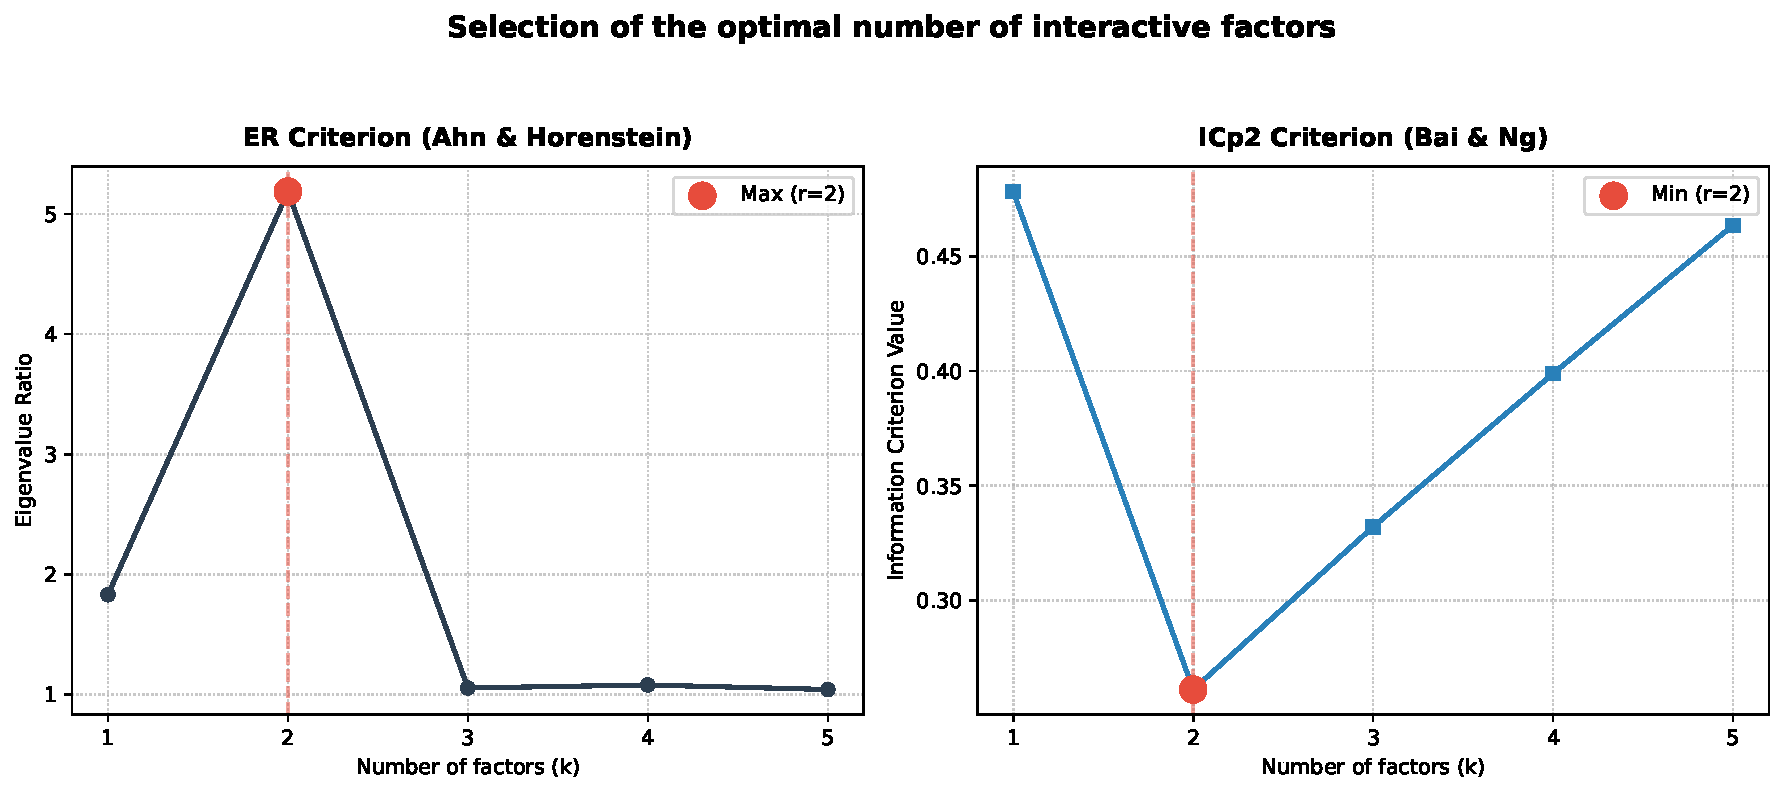
\includegraphics[width=0.85\textwidth]{figures/factor_selection.pdf}
\caption{ER (Ahn-Horenstein) and $IC_{p2}$ (Bai-Ng) factor-count criteria
for Model 3, as returned by
\texttt{model3.plot\_factor\_selection(mode='graph')} on the bundled
\texttt{df\_ife\_panel.csv} dataset. Both criteria peak/trough at $r=2$.}
\label{fig:factorselection}
\end{figure}

\note{Models 1--3 (uncollapsed, 379 instruments) converge within the
default \texttt{ife\_max\_iter=30}. Model 4 (\texttt{collapse=True}) hits
the 30-iteration cap on this dataset -- the script prints
\texttt{Warning: convergence not achieved after 30 iterations} and still
returns the last iterate, per the convergence caveat of
Section~\ref{sec:ifecaveats}. This behavior is a property of the bundled
example itself, not a curated success case. Raise \texttt{ife\_max\_iter} if
your own data needs a tighter convergence guarantee.}

\subsection{Bundled datasets}

\begin{lstlisting}[style=pystyle]
from pyxtabond2 import list_datasets
list_datasets()
\end{lstlisting}

\begin{longtable}{@{}p{0.32\linewidth}p{0.65\linewidth}@{}}
\toprule
\textbf{File} & \textbf{Description} \\
\midrule
\endhead
\texttt{df\_panel.csv} & Macro panel (Country/Year; Growth, Capital,
  Labor, Wage, Investment, Ide) used throughout the Quick Start and
  \texttt{examples.py}. \\
\texttt{df\_ife\_panel.csv} & Panel with a genuine multifactor error
  structure, used by \texttt{ife\_exemples.py} and for exercising
  \texttt{r}/\texttt{r='auto'} generally. \\
\bottomrule
\end{longtable}

\newpage
\bibliographystyle{plainnat}
\bibliography{references}

\end{document}
